\subsection{Erreichte Ergebnisse}\label{subsec:erreichte-ergebnisse}

Wie bereits im vorherigen Kapitel erwähnt, werden viele Funktionen
der Testinfrastruktur in dieser Arbeit nicht näher erläutert. Es ist
jedoch sinnvoll, einen Überblick über die bisherigen Möglichkeiten
und Ziele des UI-Tests zu geben.

\subsubsection{Einrichtung einer UI-Testumgebung}

Eine grundlegende Testumgebung wurde erstellt, um die Implementierung
zukünftiger UI-Tests zu ermöglichen. In dieser Testumgebung wurden die
Funktionen Login, Registrierung, Abruf der Noten und Einschreibung in
Prüfungen getestet. Diese Tests funktionieren für \gls{jexam_2009} (nur
der Login-Test funktioniert auch für \gls{jexam_new}). Da sich \gls{jexam_new}
noch in der Entwicklung befindet, verfügt die getestete Version noch
nicht über alle Funktionen, die getestet werden sollen.  Die Tests
wurden so geschrieben, dass sie auf beiden Plattformen funktionieren.
Es ist jedoch möglich, dass in Zukunft noch Anpassungen vorgenommen
werden müssen (dieses Problem wird im Auswertungsteil dieser Arbeit
ausführlich behandelt). Das ursprüngliche Ziel, eine Testsuite für
\gls{jexam_new} zu erstellen und gleichzeitig \gls{jexam_2009} auf
einmal zu testen, wurde erreicht. Die UI-Testumgebung kann nun
verwendet und verbessert werden, um die anderen zahlreichen Funktionen
von jExam zu testen.

\subsubsection{Testdurchführungsbericht}
Nach der Ausführung der UI-Tests generiert die Testumgebung eine
HTML-Seite, die einen detaillierten Bericht über die Ausführung
der Tests liefert (siehe \autoref{subsubsec:extent}). Dies ermöglicht es
Ihnen, die Ausführung der Tests zu überwachen und mögliche Fehler
zu erkennen.

\begin{figure}[H]
    \centering
    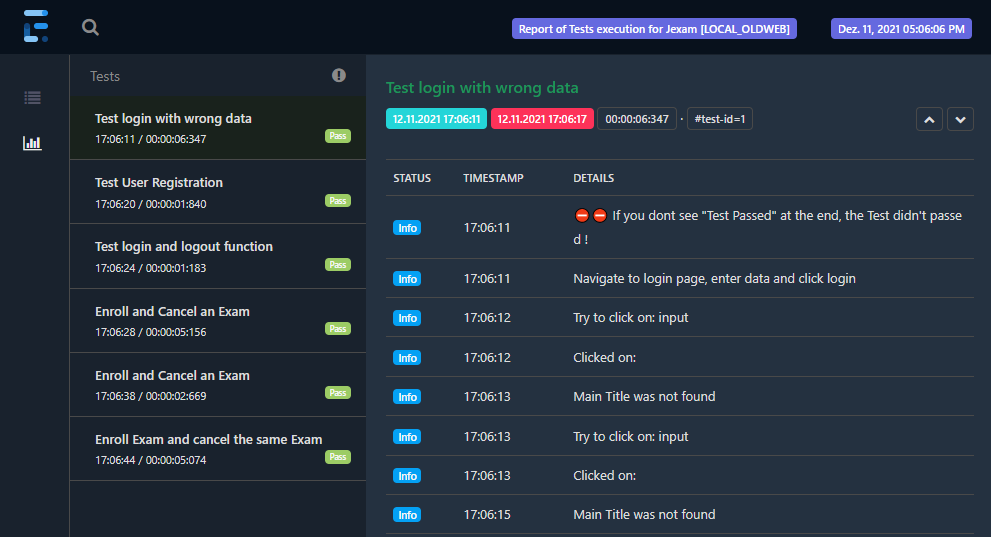
\includegraphics[scale=0.6]{images/ExtentReport}
    \caption{Extent Report HTML Page} \label{fig:ext-rep}
\end{figure}
\subsubsection{Zusätzliche Funktionalitäten}

Die UI-Testumgebung verfügt über mehrere Ausführungsmodi.
Sie ermöglicht es, die Tests lokal und remote in einem Docker-Container
auszuführen und den Prozess der Testausführung
vollständig zu automatisieren.


Die lokale Ausführung wird in der Regel bei der Implementierung
der Tests verwendet. Sie ermöglicht es, schnell zu testen, ob die
Tests korrekt funktionieren, ohne dass sie in einem Container
ausgeführt werden müssen. Dies führt zu einer erheblichen Zeitersparnis
bei der Implementierung. Der Local Run Mode bietet auch die
Möglichkeit, Tests im \gls{headless}-Modus auszuführen. \gls{headless} bedeutet,
dass die Selenium-Tests mit einem \gls{headless}-Browser ausgeführt werden.
Er funktioniert wie ein typischer Browser, jedoch ohne
Benutzeroberfläche, welcher sich für automatisierte Tests hervorragend eignet.
Der lokale Run Mode verwendet einen WebDriverManager. Dies ist sehr
nützlich, da es das Problem der Versionierung von Webdrivern löst.
Der Tester muss nicht mehr einen Webdriver auf seinen Computer
herunterladen, sondern kann den WebdriverManager verwenden, um
auf einen bereits konfigurierten und sofort einsatzbereiten Driver
zuzugreifen.

Der Remote-Modus ermöglicht die Ausführung von Tests in
Docker-Containern mithilfe des Selenium-Hubs (dieses Konzept wird
im Kapitel über die Docker-Infrastruktur behandelt). Dies ist die
Methode, die für eine vollautomatische Ausführung von UI-Tests
verwendet wird. Der Remote-Modus ist so konfiguriert, dass er die
aktuellste Version des RemoteWebDrivers verwendet (in einem
Docker-Container enthalten und mit dem Selenium-Hub verbunden).



Die beiden Testmodi ermöglichen die Durchführung von Tests unter
Verwendung der Browser Chrome und Firefox.